\section{Data Generation}
\label{sec:data_gen}
For our data generation framework, we introduce two implementations to generate scaled up datasets: Local and distributed.
Both implementations maintain data and error statistics. 
The framework contains full pipelines consisting of the following generalized steps:

\begin{itemize}
    \item Read clean and dirty data.
    \item Data analysis and error classification.
    \item Scale up the clean data by replication.
    \item Generate errors and merge with the scaled clean data.
    \item Save generated dirty dataset.
    \item Generate validation report.
\end{itemize}

\subsection{Local Data Generation}
\label{sec:local_generator}
\tikzset{bb/.style={draw, inner sep=2.5mm, rounded corners}}
\tikzset{
    ultra thin/.style= {line width=0.1pt},
    very thin/.style=  {line width=0.2pt},
    thin/.style=       {line width=0.4pt},
    semithick/.style=  {line width=0.6pt},
    thick/.style=      {line width=0.8pt},
    very thick/.style= {line width=1.2pt},
    ultra thick/.style={line width=1.6pt}
}

\begin{figure}
    \centering
    
    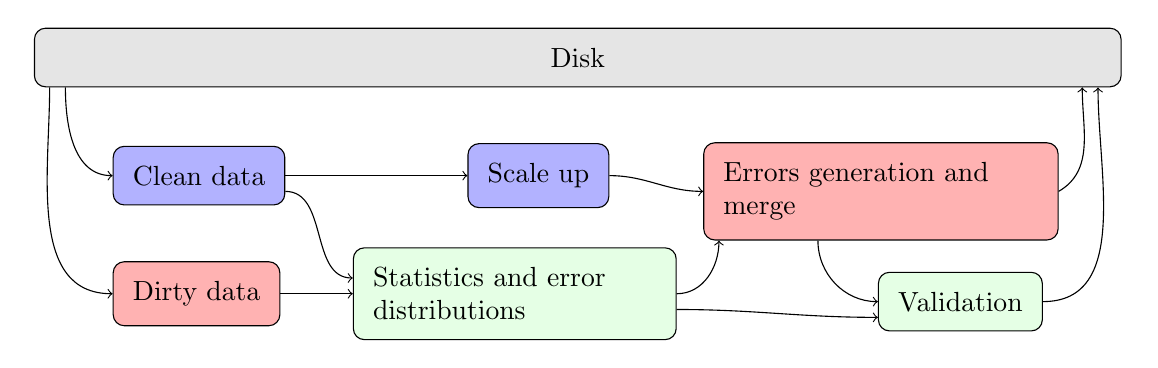
\begin{tikzpicture}[]
    \node[bb, text width=13.3cm, align = center, fill=black!10](disk){Disk};
    
    \node[bb, anchor = west, fill=blue!30] (clean) at ([yshift=-1.5cm, xshift = 1cm] disk.west) {Clean data};
    \node[bb, anchor = west, fill=red!30] (dirty) at ([yshift=-3cm, xshift = 1cm] disk.west) {Dirty data};
    
    \node[bb, text width=3.6cm, fill=green!10] (stats) at ([yshift=-3.0cm, xshift = -0.8cm] disk) {Statistics and error distributions};
    
    \node[bb, fill=blue!30] (scale_up) at ([yshift=-1.5cm, xshift = -0.5cm] disk) {Scale up};
    
    \node[bb, fill=red!30, text width=4.0cm, anchor = east] (errors) at ([yshift=-1.7cm,xshift= -0.8cm] disk.east) {Errors generation and merge};
    
    \node[bb,  anchor=east, fill=green!10] (validation) at ([yshift=-3.1cm, xshift=-1cm] disk.east) {Validation};
    
    \draw[->] ([xshift=0.4cm]disk.south west) to[out = -90, in = 180] (clean);
    \draw[->] ([xshift=0.2cm]disk.south west) to[out = -90, in = 180] (dirty);
    
    \draw[->] ([]clean.east) to[out = 0, in = 180] (scale_up);
    
    \draw[->] ([yshift=-0.2cm]clean.east) to[out = 0, in = 180] ([yshift=0.2cm] stats.west);
    
    \draw[->] ([]dirty.east) to[out = 0, in = 180] (stats);
    
    \draw[->] ([]scale_up.east) to[out = 0, in = 180] (errors);
    
    \draw[->] ([]stats.east) to[out = 0, in = -90] ([xshift=0.2cm]errors.south west);
    
    \draw[->] ([]errors.east) to[out = 30, in = -90] ([xshift=-0.5cm]disk.south east);
    
    \draw[->] ([]validation.east) to[out = 0, in = -90] ([xshift=-0.3cm]disk.south east);
    
    \draw[->] ([xshift=-0.8cm]errors.south) to[out = -90, in = 180] ([]validation.west);
    
    \draw[->] ([yshift=-0.2cm]stats.east) to[out = 0, in = 180] ([yshift=-0.2cm]validation.west);
    
    \end{tikzpicture}
    
    \caption{\label{fig:data_gen_local}Local data generator}
\end{figure}

First, for scaling to in-memory sizes there is a local data generator execution that consists of the following steps that are also shown in Figure~\ref{fig:data_gen_local}:

\textbf{Read:} 
Reading of clean and dirty datasets is done via Pandas DataFrames. 
Pandas is chosen for its flexibility, rich API and simplicity. 
An important part of the reading is detecting the schema.
Pandas has a schema detection that allows reading dirty data while handling features with different data types. 
Python in general supports collections that may contain heterogeneous data types. 
These properties together allow the creation of a save schema for the dirty data.
On the other hand, the automatic schema detection is not always precise, and integer cases can be detected as floats. 
Therefore, for the clean data, custom schema detection is applied. 
A sample of the data is extracted and analyzed for fine-grained data types. 

\textbf{Error analysis:} 
Error analysis is performed on the clean and dirty datasets together.
First, distinct values of actual data are aggregated, and a binary mask (of dirty dataset dimension) of differences between clean and dirty datasets is created.
The mask allows the framework to know the ratio and exact number of errors introduced in each feature, and to track detected and undetected errors. 
Errors are analyzed in a particular sequence, since if a cell was classified as error of one type, it can not contain any other error types, this is based on the simplifying assumption that there are no compound errors.
First, missing values are detected using the Pandas \textsc{isnull()} method. 
Second, outliers are detected by interquartile range (IQR) and by distribution. 
Formula~\ref{eq:is_outlier_iqr} uses IQR, Formula~\ref{eq:outlier_iqr}, to define lower and upper limits, while Formula~\ref{eq:is_outlier_std} relies on standard deviation, Formula~\ref{eq:std}. 
Lower and upper limits are stored, and then reused during error generation. 
Third, dirty data is inspected for replacements. 
Replacements are cells that differ from the clean dataset, but still belong to a clean distinct values set.
Fourth, to find swaps between features, the framework computes row sums utilizing the binary difference mask. 
For rows with more than 2 errors, faulty cells are checked for swaps using an all-pairs comparison of dirty cells with clean values. 
For simplicity during error generation, swaps are divided into numerical (between 2 numerical features) and mixed (between string and any other feature), since swaps between string and numerical features violate schema integrity.
Finally, all remaining erroneous \emph{string} feature values are classified as a typo.

\begin{equation}
\label{eq:outlier_iqr}
\textsc{IQR} = \textsc{Q}(0.75) - \textsc{Q}(0.25)  
\end{equation}

\begin{equation}
\label{eq:is_outlier_iqr}
\textsc{IQRO}(v) =  v < \textsc{Q}(0.25) - 1.5 \cdot \textsc{IQR} \ \cup \  v >  \textsc{Q}(0.75) + 1.5 \cdot \textsc{IQR}
\end{equation}

\begin{equation}
    \label{eq:std}
    \textsc{STD}(x) = \sqrt{\frac{\sum_{i=1}^{N}(x_{i}-\mu)^{2}}{N}}
\end{equation}

\begin{equation}
\label{eq:is_outlier_std}
\textsc{STDO(v)} = v < \overline{a} - k \cdot \textsc{STD} \ \cup \ v > \overline{a} + k \cdot \textsc{STD} 
\end{equation}

\textbf{Analysis of statistical properties:} 
Statistics analysis is performed by computing univariate statistics such as min, max, mean, variance, kurtosis and skeweness are computed for both clean and dirty datasets.
When scaling the dataset, the framework strives towards maintaining these statistics at two steps.
First, when scaling the clean dataset, the statistics of the clean dataset are maintained. 
Second, when introducing errors, the detected errors and their distribution are preserved.
To reflect a realistic dataset, Schlosser~\cite{HassNSS1995} and Hasso Stokes~\cite{HassS1998} distinct item estimators are used. 
The dirty dataset is used as a sample of the generated. It is assumed that depending on the distribution of the distinct errors in the dirty dataset, more or an equivalent number of distinct values are introduced when scaling the data.

\textbf{Scaling up:} 
Scaling up clean data while preserving statistics is challenging, especially if applied at random. 
For instance, in a column with all unique values, the probability of selecting all values at least once is low when scaling factor is small. 
It is similar to the rolling dice with 6 unique sides. 
Scaling to 2x is equivalent to rolling 6 unique sides at least once with 12 trials.
To avoid this inconsistency, we chose to scale up by replication. 
If the scaling factor is a floating point number, then the integer part is replicated, and the remaining floating part is sampled randomly from the clean data.

\begin{algorithm}[!t]
    \caption{Local Error Generation Algorithm}\label{alg:local_generator}
    \begin{algorithmic}[1] 
        \REQUIRE{Error distribution $\mat{err\_dist}$, scaled dataset $\mat{data}$, scaling factor $scaling\_factor$, schema of the dirty dataset $dirty\_schema$}
	  \ENSURE{New error distribution $\mat{new\_err\_dist}$, scaled dataset $\mat{data}$}
	  
	  \COMMENTLINE{a) create a pool to introduce mv, typos, replacements, and indices for outliers}
	  
	  \STATE $\mat{pool} \leftarrow \text{Pool}(\#CPU)$
	  \FOR{$col$ \textbf{in} $\text{data.columns}$} {
	    \STATE $kwargs \leftarrow [\mat{\text{data}}[col], \mat{\text{err\_dist}}, \mat{\text{new\_err\_dist}}, scaling\_factor, col]$ 
        \STATE $\text{tasks.append(\mat{pool}.apply\_async(\textsc{get\_errors\_in\_col},} kwargs\text{)}$ 
      }\ENDFOR 
      
      \COMMENTLINE{b) execute tasks and modify new error distribution}
	  \STATE $\mat{new\_err\_dist} \leftarrow \text{\textsc{ErrorDistribution}(dirty\_schema, \mat{data}.row, \mat{data}.col)}$
	  \FOR{$task$ \textbf{in} $\text{tasks}$} {
        \STATE $dist\_changes, col\_name, \mat{updated\_col} \leftarrow task\text{.get()}$ 
        \STATE $\mat{new\_err\_dist}.\textsc{update}(dist\_changes, col\_name)$ 
        \STATE $\mat{data}[col] \leftarrow \mat{updated\_col}$ 
      }\ENDFOR 
      
      \COMMENTLINE{c) introduce numerical swaps}
      \STATE $\mat{data}, \mat{new\_err\_dist} \leftarrow \textsc{add\_swaps}(\mat{data}, \mat{err\_dist}, \mat{new\_err\_dist})$ 
      
      \COMMENTLINE{d) introduce outliers based on indices created earlier}
      \STATE $\mat{data}, \mat{new\_err\_dist} \leftarrow \textsc{add\_swaps}(\mat{data}, \mat{err\_dist}, \mat{new\_err\_dist})$ 
      
      \FOR{$col$ \textbf{in} $\text{data.columns}$} {
        \STATE $dist\_changes, col\_name, \mat{updated\_col} \leftarrow \textsc{add\_outliers}(\mat{data}, \mat{err\_dist}, \text{new\_err\_dist.outlier\_indices})$ 
        \STATE $\mat{new\_err\_dist}.\textsc{update}(dist\_changes, col\_name)$ 
        \STATE $\mat{data}[col] \leftarrow \mat{updated\_col}$ 
      }\ENDFOR 
      
      \COMMENTLINE{e) introduce mixed swaps}
      \STATE $\mat{data}, \mat{new\_err\_dist} \leftarrow \textsc{add\_swaps}(\mat{data}, \mat{err\_dist}, \mat{new\_err\_dist})$ 
      
      \RETURN $\mat{new\_err\_dist}, \mat{data}$
    \end{algorithmic}
\end{algorithm}


\begin{algorithm}[!t]
    \caption{\textsc{get\_errors\_in\_col Algorithm}}\label{alg:local_get_errors_in_col}
    \begin{algorithmic}[1] 
        \REQUIRE{Error distribution $\mat{err\_dist}$, new error distribution $\mat{new\_err\_dist}$, scaled dataset $\mat{data}$, scaling factor $scaling\_factor$}
	  \ENSURE{New error distribution $\mat{new\_err\_dist}$, scaled dataset $\mat{data}$}
	  
	  \STATE $\mat{pool} \leftarrow \text{Pool}(\#CPU)$
	  \FOR{$col$ \textbf{in} $\text{data.columns}$} {
        \STATE $\text{tasks.append(\mat{pool}.apply\_async(\textsc{get\_errors\_in\_col})}$ 
      }\ENDFOR 
      
      \COMMENTLINE{b) execute tasks and modify new error distribution}
	  \STATE $\mat{new\_err\_dist} \leftarrow \text{\textsc{ErrorDistribution}(dirty\_schema, \mat{data}.row, \mat{data}.col)}$
	  
      
      \COMMENTLINE{c) introduce numerical swaps}
      \STATE $\mat{data}, \mat{new\_err\_dist} \leftarrow \textsc{add\_swaps}(\mat{data}, \mat{err\_dist}, \mat{new\_err\_dist})$ 
      
      \COMMENTLINE{d) introduce outliers based on indices created earlier}
      \STATE $\mat{data}, \mat{new\_err\_dist} \leftarrow \textsc{add\_swaps}(\mat{data}, \mat{err\_dist}, \mat{new\_err\_dist})$ 
      
      \FOR{$col$ \textbf{in} $\text{data.columns}$} {
        \STATE $dist\_changes, col\_name, \mat{updated\_col} \leftarrow \textsc{add\_outliers}(\mat{data}, \mat{err\_dist}, \text{new\_err\_dist.outlier\_indices})$ 
        \STATE $\mat{new\_err\_dist}.\textsc{update}(dist\_changes, col\_name)$ 
        \STATE $\mat{data}[col\_name] \leftarrow \mat{updated\_col}$ 
      }\ENDFOR 
      
      \COMMENTLINE{c) introduce mixed swaps}
      \STATE $\mat{data}, \mat{new\_err\_dist} \leftarrow \textsc{add\_swaps}(\mat{data}, \mat{err\_dist}, \mat{new\_err\_dist})$ 
      
      \RETURN $\mat{new\_err\_dist}, \mat{data}$
    \end{algorithmic}
\end{algorithm}


\textbf{Error generation and introduction:} 
Error generation and introduction is done column wise, and is presented in Algorithm~\ref{alg:local_generator}. 
Since the main workload of the framework is in this phase, each column is processed in parallel, with the exception of multi column errors such as swaps.
Typos, missing values and replacements are added to the scaled dataset in the first iteration as shown in Algorithm~\ref{alg:local_get_errors_in_col}.
For missing values and typos the distinct item sets and frequencies are gathered from the error analysis and statistics phases. 
To maintain the frequencies of missing values and typos, existing missing values and typos are scaled up, and number of new distinct missing values and typos is estimated by Schlosser \cite{HassNSS1995} and Hasso Stokes \cite{HassS1998} estimation algorithms.
Existing missing value and typo frequencies are scaled by the scaling factor. 
Additionally, a specific number of new unique values is generated, this number is estimated as described in the previous paragraph.
The number of occurrences of a new unseen unique value is computed similar to n-gram smoothing techniques. 
The new frequency of unseen values is defined by Laplace smoothing "add-one" to avoid the zero-frequency problem.
The zero-frequency problem: If an individual class label is missing, then the frequency-based probability estimate will be zero.
To introduce the errors into the data, a vector with shuffled random indices is allocated and then utilized. 
For each unique error type a random sample of indices is extracted and then applied to the scaled dataset.
Replacements are added using earlier created dictionaries of original and replaced values, and their frequencies.
Cells to modify are filtered, then a sub-fraction is randomly sampled and corrupted.
Since replacements do not introduce new distinct items, no additional computations are necessary.
Similarly, swaps are done by filtering two columns and randomly choosing rows to exchange. 
The number of rows to modify is computed from the original number of swaps and scaling factor.
To choose not already modified values for replacements and swaps, indices of modified cells are stored and then \textsc{random\_except} method is used.
This method returns random row indices that are not in the given list of indices.
The last step is the addition of outliers. 
They are applied at the end of the sequence because, if applied correctly, they can scale the mean of the new scaled dataset to the desired dirty mean through the technique described in Section~\ref{sec:error_types}. 
Outliers are also introduced to columns in a parallel manner, Algorithm~\ref{alg:local_generator}.

\textbf{Write:}  
The generated dataset is saved immediately after the error generation. It is written to the disk in comma-separated values (CSV) format. 
The dataset is saved before validation to ensure that we have the generated data, even if validation fails or concludes invalid generation.


\textbf{Validation:} 
The last stage of the framework is the validation of the generated dataset. 
It is done by comparing the statistics of the original dirty and generated datasets, the details are described in Section~\ref{sec:validation}.
The error distribution of the generated dataset is stored while generating and introducing the errors.
The univariate statistics are computed after the full generation is finished.
Both univariate statistics and error distribution are used for the validation. 
Additionally, all statistics are saved to files.

\textbf{Limitations of the local execution:} 
The Pandas DataFrames are relatively slow. Pandas is written in C, and switching between C and Python takes time, especially for mathematical computations and data retrieval.
Another limitation is the in-memory computation. This means that data can not be scaled above memory of a single machine.
Third, there is potential for more parallelization of different parts of the local execution, but the parts already parallelized include the critical parts.


\subsection{Distributed Data Generation}
\label{sec:distributed_generator}

The distributed generator is for scaling to larger sizes of data that exceeds local memory restrictions.
It consists of the following steps that are also shown in Figure~\ref{fig:data_gen_dist}:

\textbf{Read:} 
Reading of clean and dirty datasets is similar to local execution. 
To compute statistics and detect schema, local Pandas DataFrames are used. 
On the other hand, the lazily evaluated Spark DataFrame is defined for further scaling up.
The schema applied to the Spark DataFrame is obtained from a schema detection of the dirty data in Spark.
This is important to avoid schema violations while introducing different from data types into clean feature.  
For instance, swaps can be introduced between numerical and string columns.

\textbf{Error analysis and statistics: } This step is equivalent to the local execution.

\textbf{Distributed scaling up:}
Scaling of the dataset in distributed mode is achieved via three different phases. 
Since Spark DataFrame is not indexed per default, to scale it up, one of the possibilities is to append DataFrame to itself, similarly to the local.
But because of Spark usability and API, it is possible to avoid concatenation by using a combination of Spark user-defined function (\textsc{UDF}) and \textsc{explode}.
First, we define a column with sequential indices. 
Then, this column is used by a \textsc{UDF} to map each existing row index to a list of new sequential row indices.
Finally, Spark \textsc{explode} utilizes these lists to "explode" (replicate) rows with a new index.

\begin{algorithm}[!t]
    \caption{Distributed Error Generation Algorithm}\label{alg:dist_generator}
    \begin{algorithmic}[1] 
        \REQUIRE{Error distribution $\mat{err\_dist}$, scaled dataset $\mat{data}$, scaling factor $scaling\_factor$, schema of the dirty dataset $dirty\_schema$}
	  \ENSURE{New error distribution $\mat{new\_err\_dist}$, scaled dataset $\mat{data}$}
	  
	  \STATE $\mat{new\_err\_dist} \leftarrow \text{\textsc{ErrorDistribution}(dirty\_schema, \mat{data}.row, \mat{data}.col)}$
	  
	  \COMMENTLINE{a) introduce replacements}
	  
	  \STATE $\mat{pool} \leftarrow \text{Pool}(\#CPU)$
	  \FOR{$col$ \textbf{in} $\text{data.columns}$} {
        \STATE $\mat{new\_err\_dist}.rep\_indices, \mat{new\_err\_dist} \leftarrow \textsc{create\_replacements\_write\_and\_join}(\mat{data}, \mat{err\_dist}, \mat{new\_err\_dist})$ 
      }\ENDFOR
	  
	  \COMMENTLINE{b) create a pool to write files with mv, typos, and outliers}
	  
	  \STATE $\mat{pool} \leftarrow \text{Pool}(\#CPU)$
	  \FOR{$col$ \textbf{in} $\text{data.columns}$} {
	    \STATE $kwargs \leftarrow [\mat{err\_dist}, \mat{new\_err\_dist}, scaling\_factor, col]$ 
        \STATE $\text{tasks.append(\mat{pool}.apply\_async(\textsc{get\_errors\_in\_col\_dist},} kwargs\text{)}$ 
      }\ENDFOR 
      
      \COMMENTLINE{b) execute tasks and modify new error distribution}
	  \FOR{$task$ \textbf{in} $\text{tasks}$} {
        \STATE $dist\_changes, col\_name \leftarrow task\text{.get()}$ 
        \STATE $\mat{new\_err\_dist}.\textsc{update}(dist\_changes, col\_name)$ 
      }\ENDFOR 
      
      \COMMENTLINE{c) read files with errors and join into data}
      \STATE $\textsc{read\_errors\_and\_join}(\mat{data}, \mat{new\_err\_dist})$ 
      
      \COMMENTLINE{d) introduce swaps}
      \STATE $\mat{data}, \mat{new\_err\_dist} \leftarrow \textsc{create\_swaps\_write\_and\_join}(\mat{data}, \mat{err\_dist}, \mat{new\_err\_dist})$ 
      
      \RETURN $\mat{new\_err\_dist}, \mat{data}$
    \end{algorithmic}
\end{algorithm}


\begin{algorithm}[!t]
    \caption{\textsc{get\_errors\_in\_col\_dist Algorithm}}\label{alg:local_get_errors_in_col_dist}
    \begin{algorithmic}[1] 
        \REQUIRE{Error distribution $\mat{err\_dist}$, new error distribution $\mat{new\_err\_dist}$, scaling factor $scaling\_factor$}
	  \ENSURE{New error distribution $\mat{new\_err\_dist}$, column name $col$}
	  
	  \COMMENTLINE{a) get typos values}
      \STATE $\mat{new\_err\_dist}.typo\_values, num\_typos \leftarrow \textsc{get\_typos}(\mat{err\_dist})$ 
	  
	  \COMMENTLINE{b) get missing values}
      \STATE $\mat{new\_err\_dist}.mv\_values, num\_mv \leftarrow \textsc{get\_mv}(\mat{err\_dist})$ 
      
      \COMMENTLINE{d) count number of outliers}
      \STATE $\mat{new\_err\_dist}.outliers\_values, num\_outliers \leftarrow \textsc{get\_outliers}(\mat{err\_dist})$ 
      
      \COMMENTLINE{e) get random indices}
      \STATE $size \leftarrow \mat{new\_err\_dist}.num\_mv + \mat{new\_err\_dist}.num\_outliers + \mat{new\_err\_dist}.num\_typos$ 
      
      \STATE $ind \leftarrow \textsc{random\_sample\_except}($
      \STATE $\ \ \ \ \ \ \ \ \ \ \ \ \ \ \ \ \ \mat{data\_c}.nrow, size, \mat{new\_err\_dist}.replacements\_indices)$ 
      
	  \COMMENTLINE{e) write to file tuples of indices and errors}
	  \STATE $\textsc{write\_ind\_err\_to\_file}(ind, \mat{new\_err\_dist})$ 
	  
      \RETURN $\mat{new\_err\_dist}, col$
    \end{algorithmic}
\end{algorithm}


\textbf{Error generation:} 
Erroneous values are generated locally using error characteristics collected from the original dirty dataset.
The values are combined with row indices to create new error locations, Algorithm~\ref{alg:dist_generator}.
Indices are chosen at random for missing values, typos and outliers, Algorithm~\ref{alg:local_get_errors_in_col_dist}, or based on the filtering of specific values for replacements and swaps.
A challenging part here is to guarantee that indices are non-intersecting. 
To achieve this property, replacements are performed first, and afterwards random indices for other errors are chosen, avoiding already used indices.
This process is parallelized to write buffered strings of error tuples to HDFS, materializing and persisting the errors introduced in the scaled dataset.
These files can also be seen as meta data.
Introducing the errors into the actual distributed scaled up dataset is done by reading errors into Spark DataFrame from HDFS, and joining the errors with the replicated clean data on synthetic index.

\textbf{Write to HFDS:} 
Writing to HDFS was initially done using csv format, similar to the local data generation.
However, utilizing Spark compression and parquet format reduced runtime significantly.

\textbf{Validation:}  
Results validation is the same as local, except Spark functions are used to aggregate statistics for comparison of the generated and original dirty datasets.
\tikzset{bb/.style={draw, inner sep=2.5mm, rounded corners}}
\tikzset{
    ultra thin/.style= {line width=0.1pt},
    very thin/.style=  {line width=0.2pt},
    thin/.style=       {line width=0.4pt},
    semithick/.style=  {line width=0.6pt},
    thick/.style=      {line width=0.8pt},
    very thick/.style= {line width=1.2pt},
    ultra thick/.style={line width=1.6pt}
}

\begin{figure}
    \centering
    
    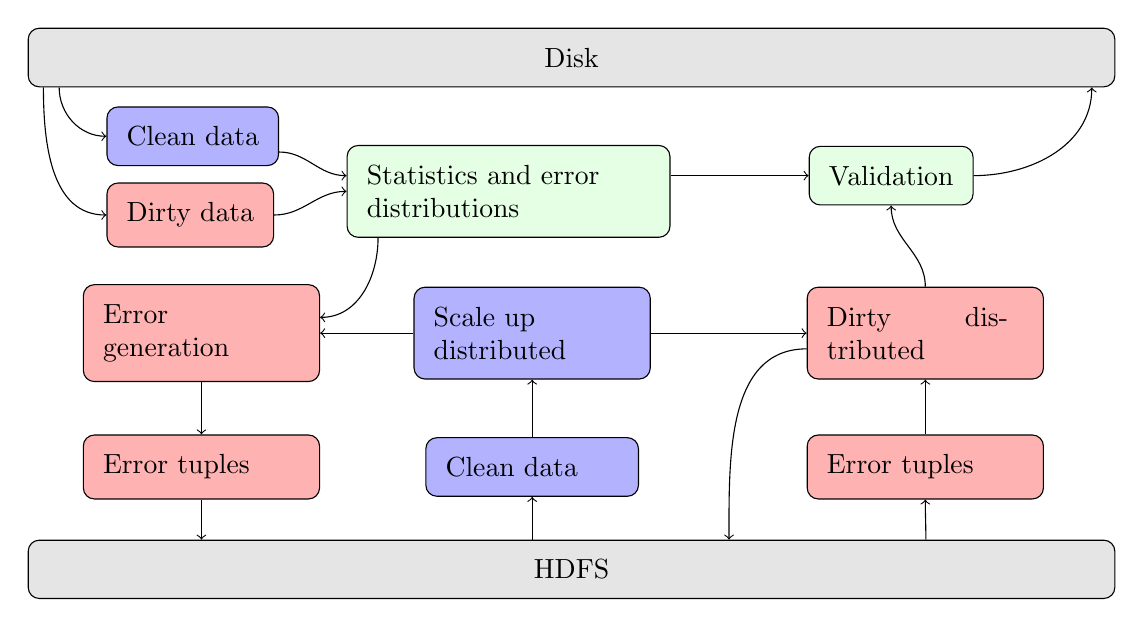
\begin{tikzpicture}[]
    \node[bb, text width=13.3cm, align = center, fill=black!10](disk){Disk};
    
    \node[bb, text width=13.3cm, align = center, fill=black!10] (hdfs) at ([yshift=-6.5cm] disk){HDFS};
    
    \node[bb, anchor = west, fill=blue!30] (clean) at ([yshift=-1.cm, xshift = 1cm] disk.west) {Clean data};
    \node[bb, anchor = west, fill=red!30] (dirty) at ([yshift=-2cm, xshift = 1cm] disk.west) {Dirty data};
    
    \node[bb, text width=2.2cm, fill=blue!30] (clean_dist) at ([yshift=-5.2cm, xshift = -0.5cm] disk) {Clean data};
    
    \node[bb, text width=3.6cm, fill=green!10] (stats) at ([yshift=-1.7cm, xshift = -0.8cm] disk) {Statistics and error distributions};
    
    \node[bb, text width=2.5cm, fill=blue!30] (scale_up) at ([yshift=-3.5cm, xshift = -0.5cm] disk) {Scale up \ \ \ \ \ \ \ \ \  distributed };
    
    \node[bb, text width=2.5cm, fill=red!30] (error_gen) at ([yshift=-3.5cm, xshift = -4.7cm] disk) {Error \ \ \ \ \ \ \ \ \ \ generation};
    \node[bb, text width=2.5cm, fill=red!30] (error_tuples) at ([yshift=-5.2cm, xshift = -4.7cm] disk) {Error tuples};
    
    % \node[bb, fill=red!30, text width=4.0cm, anchor = east] (errors) at ([yshift=-1.7cm,xshift= -0.8cm] disk.east) {Errors generation and introduction};
    
    \node[bb,  anchor=east, fill=green!10] (validation) at ([yshift=-1.5cm, xshift=-1.8cm] disk.east) {Validation};
    
    \node[bb,  anchor=east, fill=red!30, text width = 2.5cm] (dirty_dist) at ([yshift=-3.5cm, xshift=6cm] disk) {Dirty \ \ \ \ \ \ \ distributed};
    
    \node[bb, anchor=east, text width=2.5cm, fill=red!30] (error_tuples_out) at ([yshift=-5.2cm, xshift = 6cm] disk) {Error tuples};
    
    
    \draw[->] ([xshift=0.4cm]disk.south west) to[out = -90, in = 180] (clean);
    \draw[->] ([xshift=-0.5cm]hdfs.north) to[out = 90, in = -90] (clean_dist);
    \draw[->] ([xshift=0.0cm]clean_dist.north) to[out = 90, in = -90] (scale_up);
    \draw[->] ([xshift=0.2cm]disk.south west) to[out = -90, in = 180] (dirty);
    
    \draw[->] ([xshift=0.4cm, yshift=-0.0cm]stats.south west) to[out = -90, in = 0] ([yshift=0.2cm]error_gen.east);
    \draw[->] ([yshift=-0.0cm]scale_up.west) to[out = 180, in = 0] ([yshift=-0.0cm]error_gen.east);
    \draw[->] ([xshift=0.0cm]error_tuples.south) to[out = -90, in = 90] ([xshift=-4.7cm]hdfs.north);
    \draw[->] ([xshift=0.0cm]error_gen.south) to[out = -90, in = 90] ([xshift=0cm]error_tuples.north);
    
    % \draw[->] ([]clean.east) to[out = 0, in = 180] (scale_up);
    
    \draw[->] ([yshift=-0.2cm]clean.east) to[out = 0, in = 180] ([yshift=0.2cm] stats.west);
    
    \draw[->] ([]dirty.east) to[out = 0, in = 180] (stats);
    
    % \draw[->] ([]scale_up.east) to[out = 0, in = 180] (errors);
    
    % \draw[->] ([]stats.east) to[out = 0, in = -90] ([xshift=0.2cm]errors.south west);
    
    % \draw[->] ([]errors.east) to[out = 30, in = -90] ([xshift=-0.5cm]disk.south east);
    
    \draw[->] ([]validation.east) to[out = 0, in = -90] ([xshift=-0.3cm]disk.south east);
    
    % \draw[->] ([xshift=-0.8cm]errors.south) to[out = -90, in = 180] ([]validation.west);
    
    \draw[->] ([yshift=0.2cm]stats.east) to[out = 0, in = 180] ([yshift=-0.0cm]validation.west);
    
    \draw[->] ([xshift=4.5cm]hdfs.north) to[out = 90, in = -90] (error_tuples_out);
    
    \draw[->] ([xshift=0cm]error_tuples_out.north) to[out = 90, in = -90] (dirty_dist);
    
    \draw[->] ([xshift=0cm]scale_up.east) to[out = 0, in = 180] (dirty_dist.west);
    
    \draw[->] ([yshift=-0.2cm]dirty_dist.west) to[out = 180, in = 90] ([xshift=2cm]hdfs.north);
    
    \draw[->] ([yshift=0cm]dirty_dist.north) to[out = 90, in = -90] ([xshift=0cm]validation.south);
    
    \end{tikzpicture}
    
    \caption{\label{fig:data_gen_dist}Distributed data generator}
    
\end{figure}
